\chapter{Literature Review}

This chapter reviews the research papers, articles, books and other relevant forms of research used in the design of the NPSC. It has been divided into the sections illustrated by \cref{fig:lit_rev}:
\begin{figure}[h!]
\centering
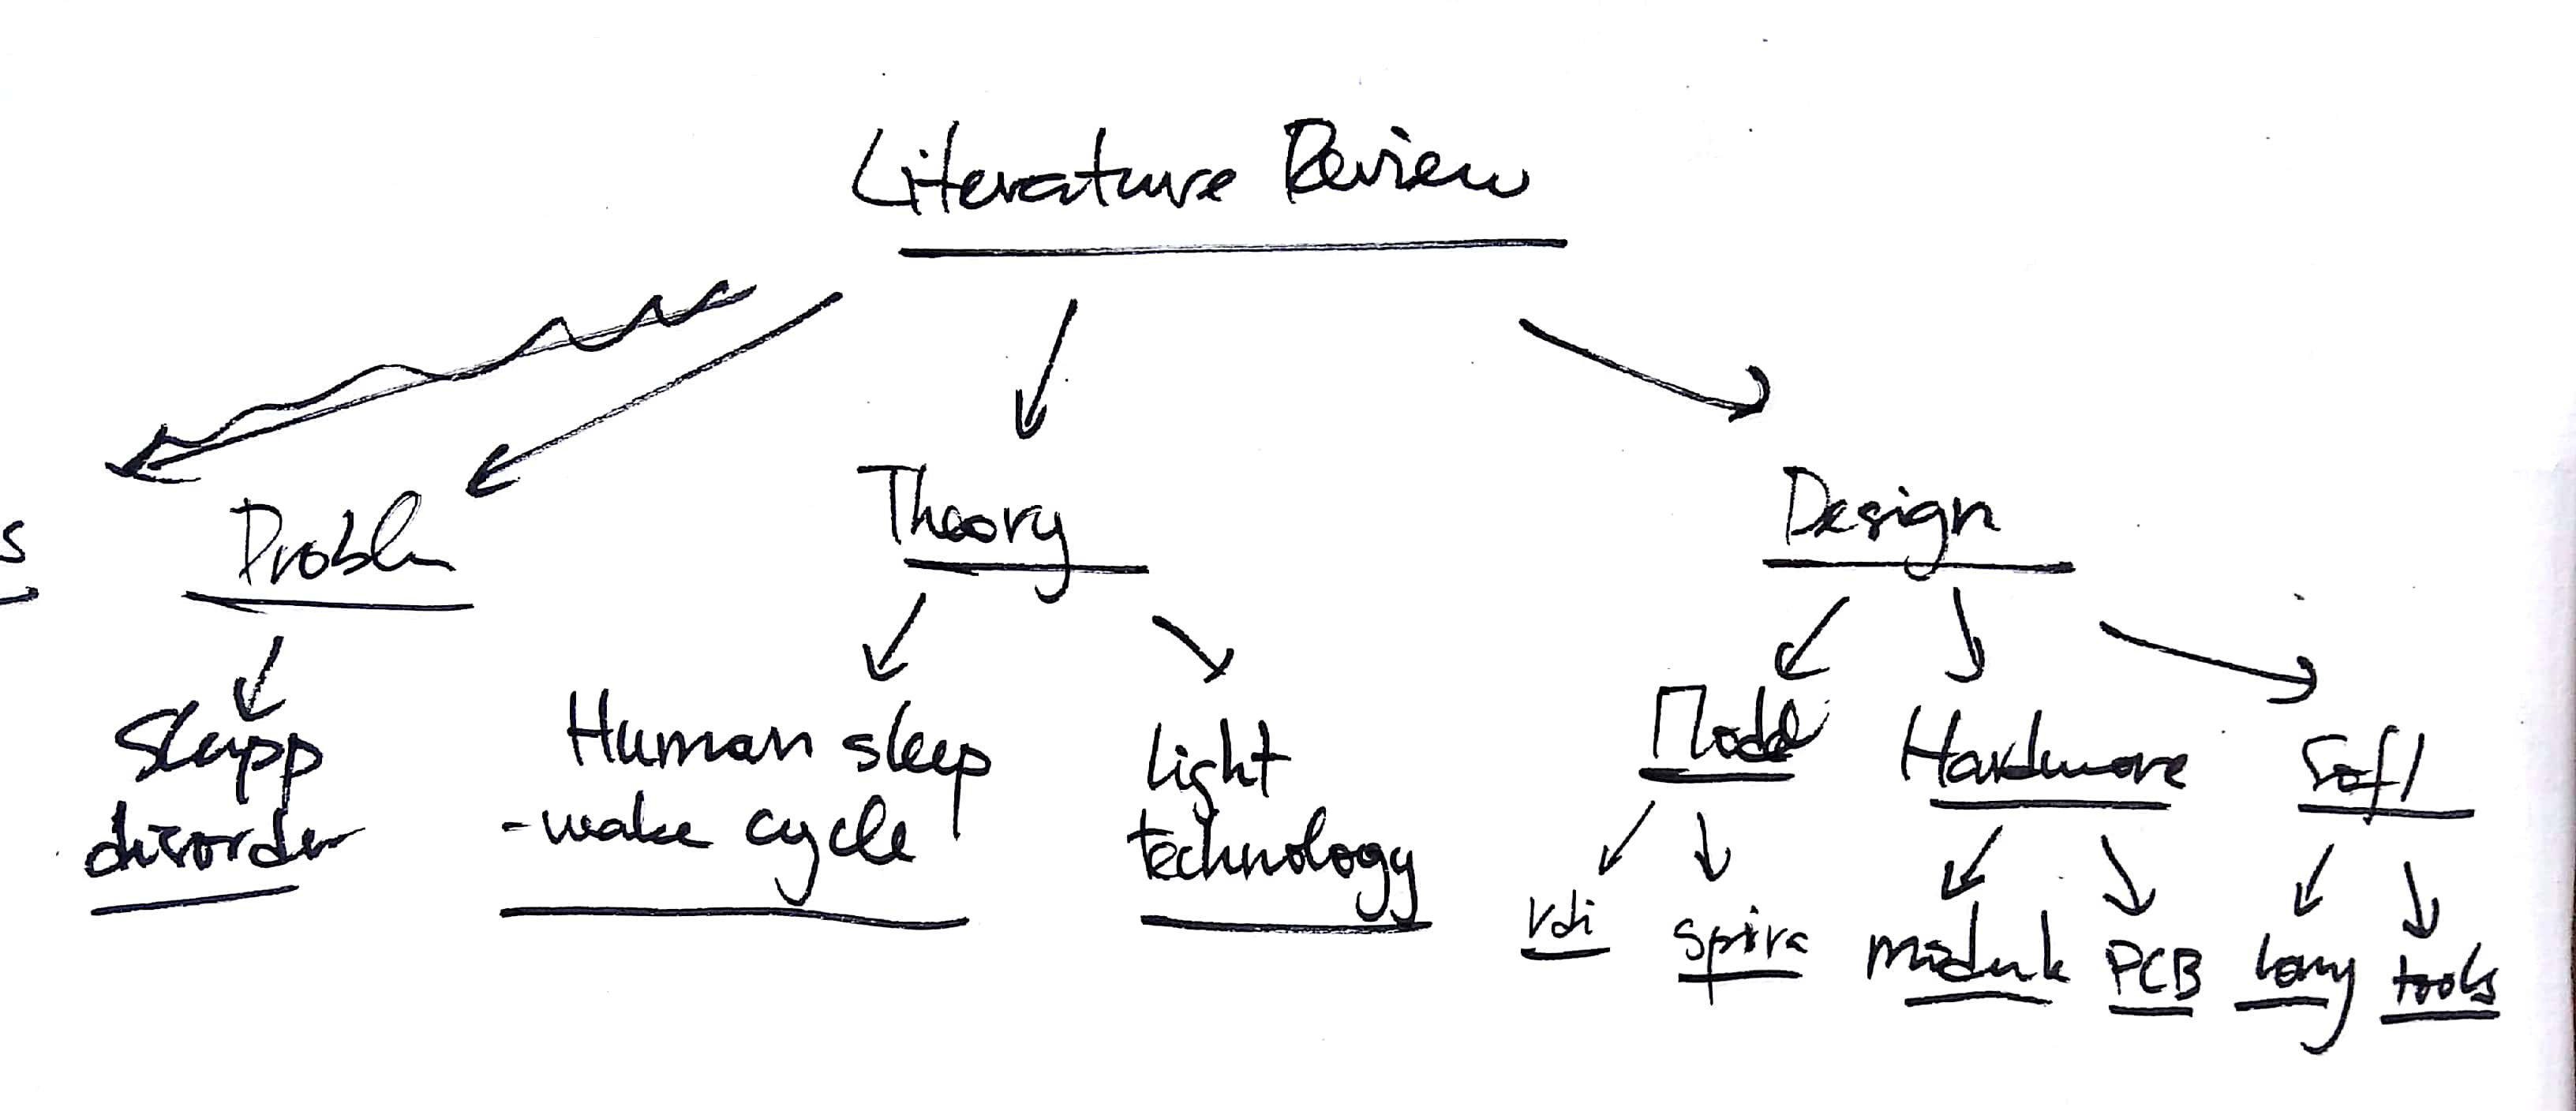
\includegraphics[scale=0.1]{lit_rev.jpg}
\caption{Overview and classification of the sections of the literature review.}
\label{fig:lit_rev}
\end{figure}
The literature review starts with an explanation of the problems to be solved, it continues by uncovering the theory behind these problems and ends with a review of the design methods, hardware components and software tools used in this project.

%%%%%%%%%%%%%%%%%%%%%%%%%%%%%%%%%%%%%%%%%%%%%%%%%%%%%%%%%%%%%%%%%%%%%%%%%%%%%%%%%%%%
% SECTION: The human sleep-wake cycle
%%%%%%%%%%%%%%%%%%%%%%%%%%%%%%%%%%%%%%%%%%%%%%%%%%%%%%%%%%%%%%%%%%%%%%%%%%%%%%%%%%%%
\section{The human sleep-wake cycle}

Human has many \say{internal clocks} among them is the master clock located in the suprachiasmatic nuclei. These internal clocks or endegenous clocks are internal mechanisms in organisms reponsible for the regulations of certain functions or activities. The master clock cheif among them, regulates the secretion of melatonin is affected by light. The creation of artifical light expecially LEDs have caused a disruption in the sleep-wake cycle. This section give an overview of the human internal clocks and how they are affected by light.

\subsection{The circadian rhythm}
Human seasonal behaviours are synchronised to the environment by \textbf{biological clocks} responsible for the creation of biological rhythms. Biological clocks which are composed of proteins that act reciprocally on the body's cells are the natural timing devices found in many organs. The discovery of the genes from these biological clocks responsible for the control of these rhythms was made by three scientists Jeffrey  C.  Hall,  Michael  Rosbash and Michael W. Young winners of the Nobel Prize in Physiology or Medicine \cite{sc2017}. Their discovery made in the 1980s led to advanced research on the role of the circadian rhythms.\\
Circadian rhythms are biological rhythms which follow the same pattern in absence of external cues (endogenous), are influenced by the presence of external stimuli (entertainable), oscillating roughly every 24h\footnote{it oxalates generally a period near 24h} over a range of physiological temperatures. In the presence of external stimuli -also known as \textit{zeitgebers}-, circadian rhythms synchronise their periodicity with these external stimuli. The zeitgebers of the circadian are the daily variation of the temperature and the dark/light cycle of the day.\\
Circadian rhythms have endogenous and exogenous components. Human placed in isolation without knowledge of the time continued exhibiting a circadian rhythm with their pacemakers notably the melatonin secretion, sleep-wake cycle, body temperature \cite{in1996}. These results prove the existence of endogenous components of the circadian rhythms as it illustrates the effects of these internal signal on the circadian rhythms. A similar study shows that when people are exposed to light at night time, a shift in their pacemakers \cite{ea2004} which is an evidence of the exogenous component of circadian rhythms. These exogenous components of the circadian rhythms have the ability affect positively and negatively our natural endogenous cycle. With light being what we are mostly daily exposed to, what is the influence of light on the circadian rhythms? 

\subsection{Internal circadian rhythms influenced by light}
Melatonin is the hormone produced by the pineal gland in the suprachiasmatic nuclei (SCN) which has a soporific effect and the ability to entertain the sleep-wake cycle. While melatonin itself is not the cause of a person sleeping, it however creates changes in a person's body that affect their sleepiness. \\
The pineal gland responsible for the secretion of the melatonin hormone is under the influence of one of the biological clocks, the master clock located in the SCN. The SCN receives visual information from the retinal-hypothalamic tract which entrains the SCN according to the photoperiod \cite{lig1994}. The SCN in turn activate a gene in the pineal cell (CREM) which produces a protein (ICER) needed for the production of melatonin. As a result, the secretion of pineal hormone melatonin tracks the light/dark cycle with its  secretion being high during the day and low during the night.  

\subsection{Quantitative and qualitative characteristics of light on melatonin production}
Many types of research have been done to understand the impact of light on the circadian rhythms especially the sleep-wake cycle. \\
Kathleen \textit{et al.} in their paper \textit{Blue light from light-emitting diodes elicits a dose-dependent suppression of melatonin in humans}\cite{bl2010}, provide details information on their finding of the effect of light on humans subject. Subjects used for the experiments were 5 males and 3 females with a mean of $23.9\pm0.5$ years, with each subject demonstrating normal colour vision. The lighting requirement was blue light of $\lambda_{max} = 469nm \pm 1nm $ with $\frac{1}{2}$ peak bandwidth$ = 26nm$ and a typical viewing distance of $35cm$. The subjects were blindfolded from midnight to 2 AM. From thereon, they were exposed to 90 min of blue light exposure followed by another dark exposure. Blood samples from the subject were taken from 2 AM at 30 min interval.From their experiment, they concluded that:
\begin{itemize}
\item \textit{Blue LED light has an increased melatonin suppression following an increase in exposure irradiance}
\item \textit{Blue LED light may have stronger suppressing effect than 4000K white fluorescent light.}
\end{itemize}
A similar study was previously made by George C. Brainard \textit{et al.} \cite{ac2001} used 72 healthy human subjects, with normal colour vision. The subjects composed of 37 females, 35 males, aged between 18 and 30 years (mean age of $24.5 \pm 0.3$ years), came from different ethnic (African, African Americans, Caucasians, Asian, Hispanic). The melatonin suppression action spectrum was formed using eight different wavelengths between $440nm$ and $600nm$ \textit{(440, 460, 480, 505, 530, 555, 575, 600)}. Using the same procedure as mentioned in the previous experiment, blood samples were taken at 30 min interval after 2 AM. The results of their research published in their paper \textit{Action Spectrum for Melatonin Regulation in Humans: Evidence for a Novel Circadian Photoreceptor} the following conclusion:
\begin{itemize}
\item \textit{Light irradiance greater or equal to $3.1 \mu W/cm^{2}$ evoke a significant melatonin supression}
\item \textit{Smaller wavelength monochromatic light have a greater change in \textit{Plasma Melatonin as Percent Change Control-Adjusted} for a fixed value of \textit{Photon density}} (\cite{ac2001} pp. 4-5).
\end{itemize}   

\subsection{Impact of light on human behaviour and sleep-wake cycle}
Among the Zeitgebers (natural phenomenon acting as a signal in the regulation of the circadian rhythm)  of the circadian rhythms, light is the major Zeitgebers and has important effects on the human sleep-wake cycle. A study on the \say{Circadian and Light Effects on Human Sleepiness-Alertness} made by Christian \textit{et al.}\cite{cir2014} shows that with nor phase lag or lead between the circadian rhythm and the sleep-wake cycle, subjective sleepiness and core body temperature have opposite behaviour (\cite{cir2014}, pp. 12, fig. 2.1). The human normal sleep-wake cycle is comprised of 8h of sleep and 16h of wakefulness \cite{is1995}. This cycle is naturally affected by the human activities but is highly influenced by light exposure. The study shows that office workers with bright blue office light have a better sleep-wake cycle than those with dim and warm office light. Furthermore, it shows that light exposure of sufficient intensity at night can reduce the secretion of melatonin with alerting response starting within the first 20mm. With the recent advance in LED technologies, humans are no longer following the natural light/dark cycle causing numerous sleep disorders. 

%%%%%%%%%%%%%%%%%%%%%%%%%%%%%%%%%%%%%%%%%%%%%%%%%%%%%%%%%%%%%%%%%%%%%%%%%%%%%%%%%%%%
% SECTION: LEDs technologies
%%%%%%%%%%%%%%%%%%%%%%%%%%%%%%%%%%%%%%%%%%%%%%%%%%%%%%%%%%%%%%%%%%%%%%%%%%%%%%%%%%%%
\section{Lighting technologies}

Light is capable of affecting the human sleep-wake cycle. However this impact can be used to reverse the negative impact of light on the sleep-wake cycle. This section introduces the different light technologies available and their use in regualting the human sleep-wake cycle. 

\subsection{Light}
The sun's electromagnetic radiation has a broad light spectrum ranging from  $100nm$ to $1mm$. After being filtered through the earth atmosphere, only certain portions of the spectrum are kept with the visible light spectrum having the maximum irradiance. Because the human circadian rhythms are automatically synchronised to the natural light-dark cycle, the characteristics of the sunlight are used as a benchmark in the emission of artificial light. These artificial lights are able to produce more or less the same wavelength as the sunlight but with much less irradiance.

\subsection{Type of light technologies}
Various light technologies have been developed over the years, their use and their usefulness in this project are detailed below. 
\subsubsection{Incandescent light}
These are the most common and least efficient light technology. It produces light by passing a high current through a wire filament producing warm light as it glows. These type of lights produce only a specific spectrum of light (warm light) besides they are not designed to be programmable. 
\subsubsection{Fluorescent light}
Light is produced by passing electricity through mercury vapour, the invisible light produced as a result of that interaction, connect with the coating of the glass emitting light. It produces all type of white light (warm, cool, daylight) with a good colour rendering. Compared to the incandescent light, it only produces one type of colour and it is not designed to be programmable.
\subsubsection{Halogen light}
It shares similarities with the incandescent light except that halogen gas is added to the glass. It produces a crisp white colour. As the previous technologies, it also produces one type of colour and it not designed to be programmed.
\subsubsection{Xeon light}
This type is another version of incandescent light with Xeon gas added to the glass instead, it produces a less yellow light. As the previous technologies, it also produces one type of colour and it not designed to be programmed.
\subsubsection{LED light}
This technology uses the passage of current through a diode to produce light. These light are very efficient and provide all sort of colour as well as cool and warm light. Moreover, their ability to work based on the passage on current allows these lights to be programmable. New LED technologies have a microcontroller which can be programmed the LEDs. 
\subsection{Light treatment of sleep disorder}
With the discovery of the effect of light on the sleep-wake cycle, electronic devices producing specific light have been used in treating patients with sleep-disorder. Advanced sleep phase disorder (ASPD) have been treated using a therapeutic approach involving chronotherapy and timed light exposure \cite{th2010}. The same concept has been used to create a home bed lamp or alarm clock facilitating the regulation of the sleep-wake cycle. \textbf{GE Sol} and \textbf{Philips}\textit{(which is actively involved in sleep-wake cycle treatment)} have created devices able to ``influence'' the human sleep-wake cycle.

\subsubsection{C by GE Sol}
\textit{C} shown in \cref{fig:c} is a ``all-in-one smart light'' \cite{gesol} which has Amazon intelligent personal assistant Alexa built in. C has a various range of colours which are manually selected based on the user preference. It is capable of communicating with GE sol devices and smartphones inserting it among the user's network of devices. Despite its high technology features and its elegant design, C remains just a bed lamp as it is not clinically proven to be helpful in regulating the user's sleep-wake cycle.
\begin{figure}[h!]
\centering
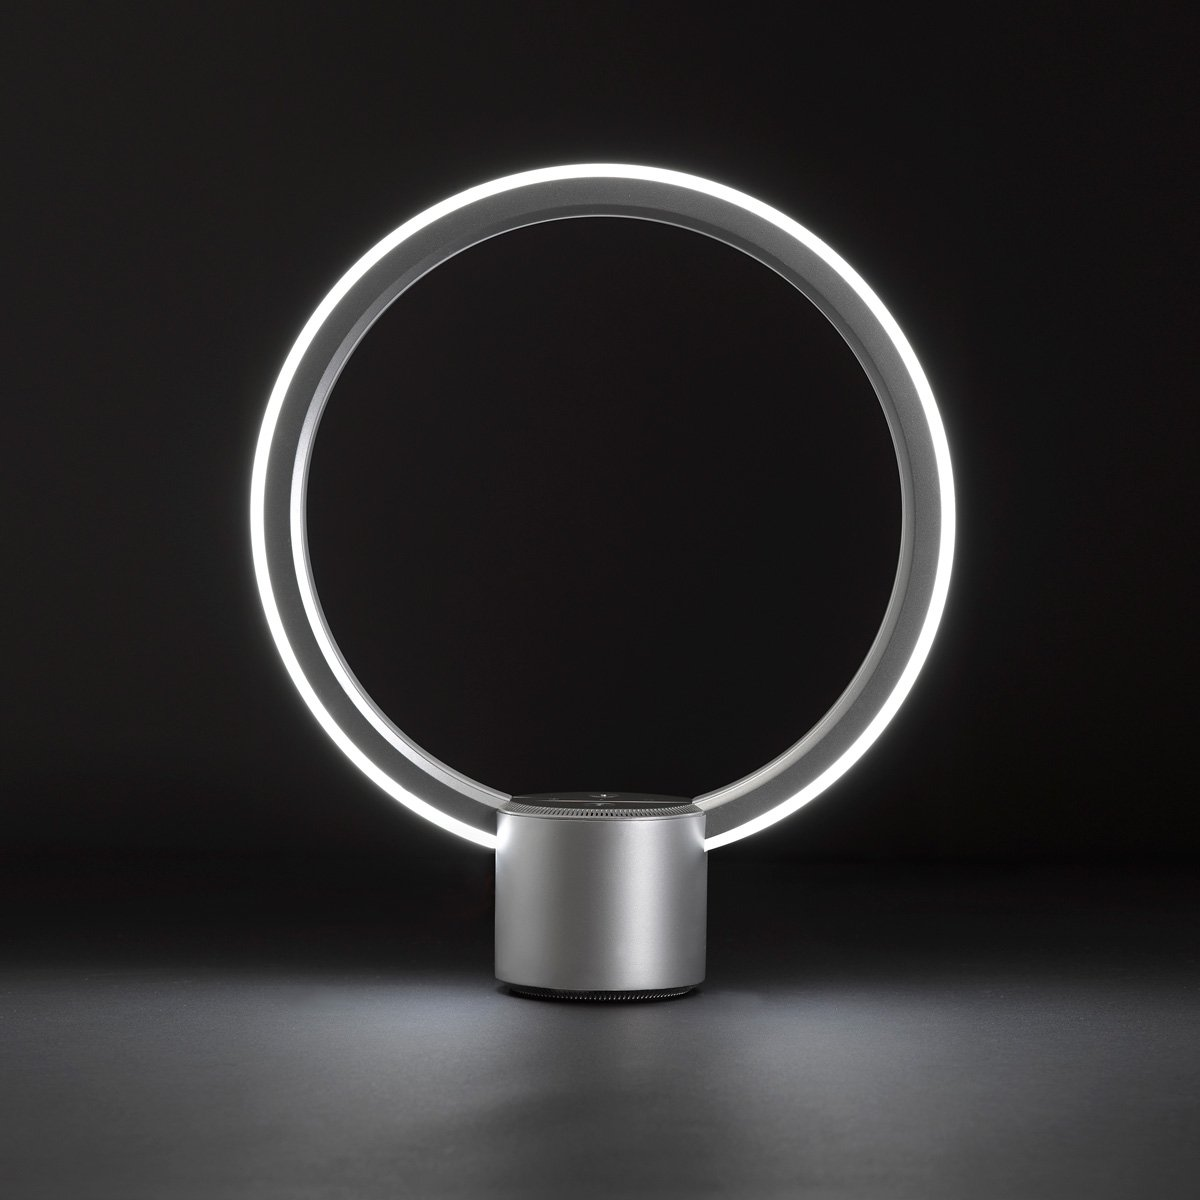
\includegraphics[scale=0.2]{sol1.jpg}
\caption{C by GE Sol, an intelligent lamp bed using Amazon Alextra.}
\label{fig:c}
\end{figure}

\subsubsection{Philips wake-up lamps}
Philips has created a broad range of wake-up lamps designed to impact the sleep-wake cycle of the users. \Cref{fig:philips1,fig:philips2} are examples of the recent versions of Philips' clocks able to simulate sunrise and sunset which last from 20 to 40 mm. These simulations vary the colour of the light following the sun's natural sunrise colour and end with a selected channel or prefered user's music. These Sleep and Wake-up lights are the only wake-up lamp clinically proven to work as stated by Philips\cite{philips}. 

\begin{figure}[h!]
\centering
\begin{minipage}[b]{0.45\textwidth}
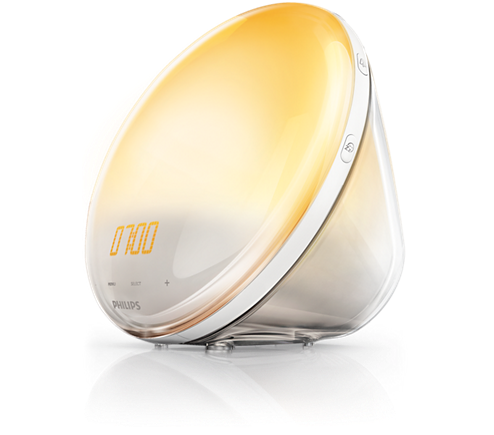
\includegraphics[scale=0.4]{philips1.png}
\subcaption[first caption.]{HF3531/60, coloured sunrise\\ simulation, 7 natural sounds, Tap\\ snooze and reading lamp, midnight\\ light function}
\label{fig:philips1}
\end{minipage}
\begin{minipage}[b]{0.45\textwidth}
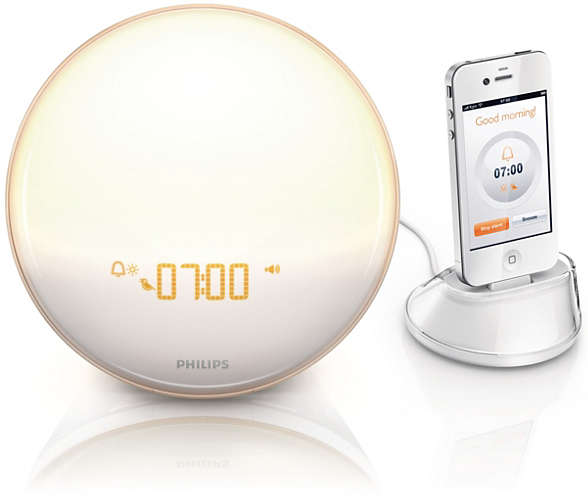
\includegraphics[scale=0.35]{philips2.jpeg}
\subcaption[second caption.]{HF3551/60, coloured sunrise simulation, 7 natural sounds, Tap snooze and reading lamp, midnight light function, Operated by iPhone App}
\label{fig:philips2}
\end{minipage}
\caption{Wake-up light by Philips}
\label{philips}
\end{figure}

\vfill
NEED SOME TRANSITION HERE 

%%%%%%%%%%%%%%%%%%%%%%%%%%%%%%%%%%%%%%%%%%%%%%%%%%%%%%%%%%%%%%%%%%%%%%%%%%%%%%%%%%%%
% SECTION: Hardware modules 
%%%%%%%%%%%%%%%%%%%%%%%%%%%%%%%%%%%%%%%%%%%%%%%%%%%%%%%%%%%%%%%%%%%%%%%%%%%%%%%%%%%%
\section{Hardware modules}
This section provides the research on the hardware technologies as well as the reasons behind the choice of some of these technologies. 

\subsection{Processors and microcontrollers}
A microcontroller is an integrated circuit which is dedicated to execute tasks of a specific application. It is physically small, cheap compared to a computer, and is designed to operate a low power consumption \cite{ho2000}.\\
Numerous microcontrollers were analysed for this project. Each manufacturer provides various range of microcontroller suitable for different applications.
The NPSC's microcontroller needs to communicate to a smartphone application wirelessly and control various external modules. While controlling the external modules, the microcontroller needs to perform processing of the sunrise and sunset patterns by continuously organising and sending data to the neopixels. In order to reduce the complexity of finding the \textit{perfect} microcontroller for the NPSC, the selection was based on the following characteristics:
\begin{itemize}
\item \textbf{Size of the FLASH:} How many lines of code can be loaded to the microcontroller?
\item \textbf{Cost}
\item \textbf{Clock speed}
\item \textbf{Community:} Does the manufacturer have a large community of developers?
\item \textbf{Bit precision:} Are we aiming at 8, 16, or 32 bits precision? 
\item \textbf{Familiarity:} How familiar are we with the microcontroller (time is a constraint)?
\item \textbf{Number of pins:} How many ports does it provide?\
\item \textbf{Extra features:} What are the built-in functionalities (wifi module, bluetooth)?
\end{itemize}

\Cref{table:micro} provides the difference between the microcontrollers selected, this table was use to make the final decision on the microcontroller selection.
\begin{table}[h!]
\centering
\caption{Comparison between specifications of the Arduino Due \cite{arduino}, the Intel Edison \cite{intel}, the Raspverry Pi Zero \cite{raspberry}, and the STM32F407VGT6\cite{stm}}
\label{table:micro}
\begin{tabular}{cp{5em}p{8em}p{5em}c}
\hline
\hline
\multirow{2}{*}{Characteristics}  & \multicolumn{4}{c}{Microcontrollers} \\  
 & \textbf{Arduino Due} & \textbf{Intel Edison} & \textbf{Raspberry Pi Zero} & \textbf{STM32F407VGT6} \\
\hline
\textbf{Clock speed} & 84MHz &  dual-core, dual-threaded 500 MHz CPU & 1GHz single core & 168 MHz\\
\textbf{Bit precision} & 32 & 32 & 32 & 32 \\
\textbf{FLASH} & 512KB & 4GB & MicroSDHC & 1MB \\
\textbf{Pins} & 54 & 40 & 40 & 82\\
\textbf{Cost} & R549.25 & R687.87 & R79.8 & R114.83\\
\hline
\hline
\end{tabular}
\end{table}

\subsection{Storage}
Storages are important in the development of embedded solutions. The \textbf{Electrical Erasable Programmable Read-Only Memory} (EEPROM) is a non-volatile memory capable of keeping its data after being powered off. There are two types of EEPROMs, serial and parallel EEPROMs. In a study made by Microship on the difference between serial and parallel EEPROM of 16KB, Tom Tyson from the Memory Product Divisions concluded that the serial EEPROM is \textit{the best option for embedded solutions requiring a small EEPROM footprint, low current and low operating voltage, the ability and ease to programme a byte at a time, and the best price-performance non-volatile memory solution available}\cite{serialvsparallel} (pp. 4).
The NPSC needs to store the user's data and the NPSC default's settings. Having a non-volatile external memory easy to program is of benefits to the NPSC.

\subsection{Wireless technology}\label{wireless_technologies}
Different types of wireless technologies allow devices to communicate to each other wirelessly. The Institute of Electrical and Electronics Engineers (IEEE) has grouped them in the 802.15 technologies. Among these are the well-known Wifi, cellular machine to machine (M2M), mesh network using ZigBee, Z-wave \ldots and Bluetooth. \\
The NPSC needs to make a wireless connection to communicate with a smartphone application. The appropriateness of the technologies tabulated in \cref{tab:wireless} for the NPSC are analysed below. 
Wifi modules are inexpensive; however, smartphones communicating with the NPSC will require being connected to the same wifi. Moreover, a web application might need to be designed as a platform for the NPSC, this will raise security issues that we would not be able to explore to the time constraint of the project. Cellular machine to machine has one main drawback, its recurring cost. As its name indicate, this technology is to send information from a machine to another machine and is not optimal for a graphic design platform\footnote{having a phone or web application that make use of this would be horrible}.  Mesh networks are optimal for interactions of device/machine of the same kind (not a requirement), the NPSC does not fall into that category. Bluetooth is designed for short-range communication (the typical distance is around $10m$  \footnote{can be increased by increasing the transmission power})being in almost all smartphones it has been extensively used by embedded systems device such as handsets, Bluetooth speakers. It has a full-duplex communication with synchronous and asynchronous channel. Using Bluetooth, the NPSC will not require any network or incur any recurring cost to the user. 

\begin{table}[h!]
\centering
\caption{Comparison between the constraints and the convenience of Wifi, M2M, Mesh network, and Bluetooth}
\label{table:wireless}
\begin{tabular}{ccc}
\hline
\hline
\textbf{Technology} & \textbf{Constraints} & \textbf{Convenience} \\
\hline
\textbf{Wifi} & Wifi network and security protocol & Yes\\ 
\textbf{M2M} & Recurring cost & No\\
\textbf{Mesh} network & Machine/Device of the same kind & No\\
\textbf{Bluetooth} & Short range & Yes\\
\hline
\hline
\end{tabular}
\end{table}

\subsection{Touch screen}
A touch-screen device can locate the position of a point of contact on its screen. 
\Cref{fig:screen} illustrates the difference between resistive and capacitive touchscreen. Resistive touch-screens are made out of many layers of which two are composed of indium-tin-oxide (ITO) which is highly resistive and transparent. By applying pressure on one of the layers, the layers come in contact creating a signal that is used to find the location of the point of contact. Capacitive touch-screens, on the other hand, make use of the conductivity of the object in contact with the screen to affect the electrostatic field between the ITO layers. Resistive touch-screens are less complex than capacitive touch-screens, thus cheaper. Additionally, because they rely on pressure, any object whether conductive or not can be used on the screen which is made to be robust. However, resistive touch-screens do not support multi-touch and have poor contrast because of the extra layer used to protect the ITO layers.\\
The NPSC need to have an onboard controller. This controller must be user-friendly, with the different features of the NPSC, a touch-screen is desirable over a controller with physical buttons. A resistive touchscreen would add to the robustness of the NPSC as a whole.   
\begin{figure}[h!]
\centering
\begin{minipage}[b]{0.45\textwidth}
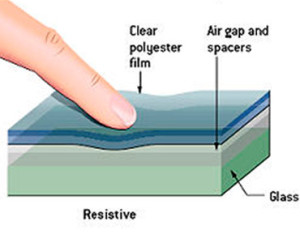
\includegraphics[scale=0.4]{resistiveTouch.jpg}
\subcaption[first caption.]{Resistive touch-screen technology\cite{resistivetouch}.}
\label{fig:resistive_screen}
\end{minipage}
\begin{minipage}[b]{0.45\textwidth}
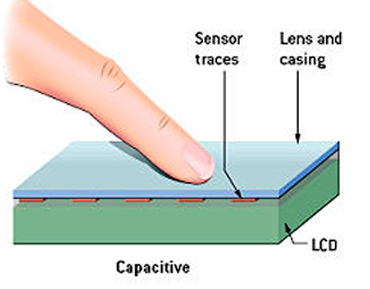
\includegraphics[scale=0.35]{capacitiveTouch.jpg}
\subcaption[second caption.]{Resistive touch-screen technology \cite{capacitivetouch}.}
\label{fig:capacitive_screen}
\end{minipage}
\caption{Touch-screen technologies. More pressure need to be applied on the resistive touch screen for location dectection.}
\label{fig:screen}
\end{figure}    

\subsection{Neopixels}\label{neopixels}
The neopixel is a programmable light source using an MCU to control an RGB or RGBW LEDs. Each colour is capable of producing 255 brightness levels resulting in 16777216 different RGB colours. 
The light characteristics of the neopixel of choice are presented in \cref{table:neopixel_specs}. The light requirement of the NPSC is the emmission of light of $460nm\pm10$ (blue light) at an illuminance of $30lux$ minimum.

\begin{table}[h!]
\centering
\caption{Light specification of the WS2812 neopixels}
\label{table:neopixel_specs}
\begin{tabular}{cp{6em}p{6em}p{6em}c}
\hline
\hline
\textbf{Emitting colour} & \textbf{Model} & \textbf{Wavelength (nm)} & \textbf{Luminous intensity (mcd)}  & \textbf{Current (mA)}\\ 
\hline
Red & 13CBAUP & 620-625 & 390-420 & 20\\
Green & 13CGAUP & 522-525 & 660-720 & 20\\
Blue & 10R1MUX & 465-467 & 180-200 & 20\\
\hline
\hline
\end{tabular}
\end{table}

The illuminance of a light source at a point is given by: 
\begin{equation}\label{eq:illuminance}
E_{v(lx)}=\frac{I_{v(cd)}}{d_m^2}
\end{equation}
\cref{eq:illuminance} is the illuminance directly in front of the light source. \textbf{Lambert's Cosine Law} says that the illuminance \textit{is directly proportional to the cosine of the angle made by the normal to the illuminated surface with the direction of the incident flux.} \cite{optical}, mathematically it means:
\begin{equation}\label{eq:lambert}
E_{v_1}=E_v*\cos(\theta)
\end{equation}
\textit{with $\theta$, the angle θ between the direction of the incident light and the surface normal}.\\
The dimension to be considered for the calculation of the illuminance of the neopixel ring are shown in \cref{fig:neopixel_ring_dimension}.
\begin{figure}[h!]
\centering
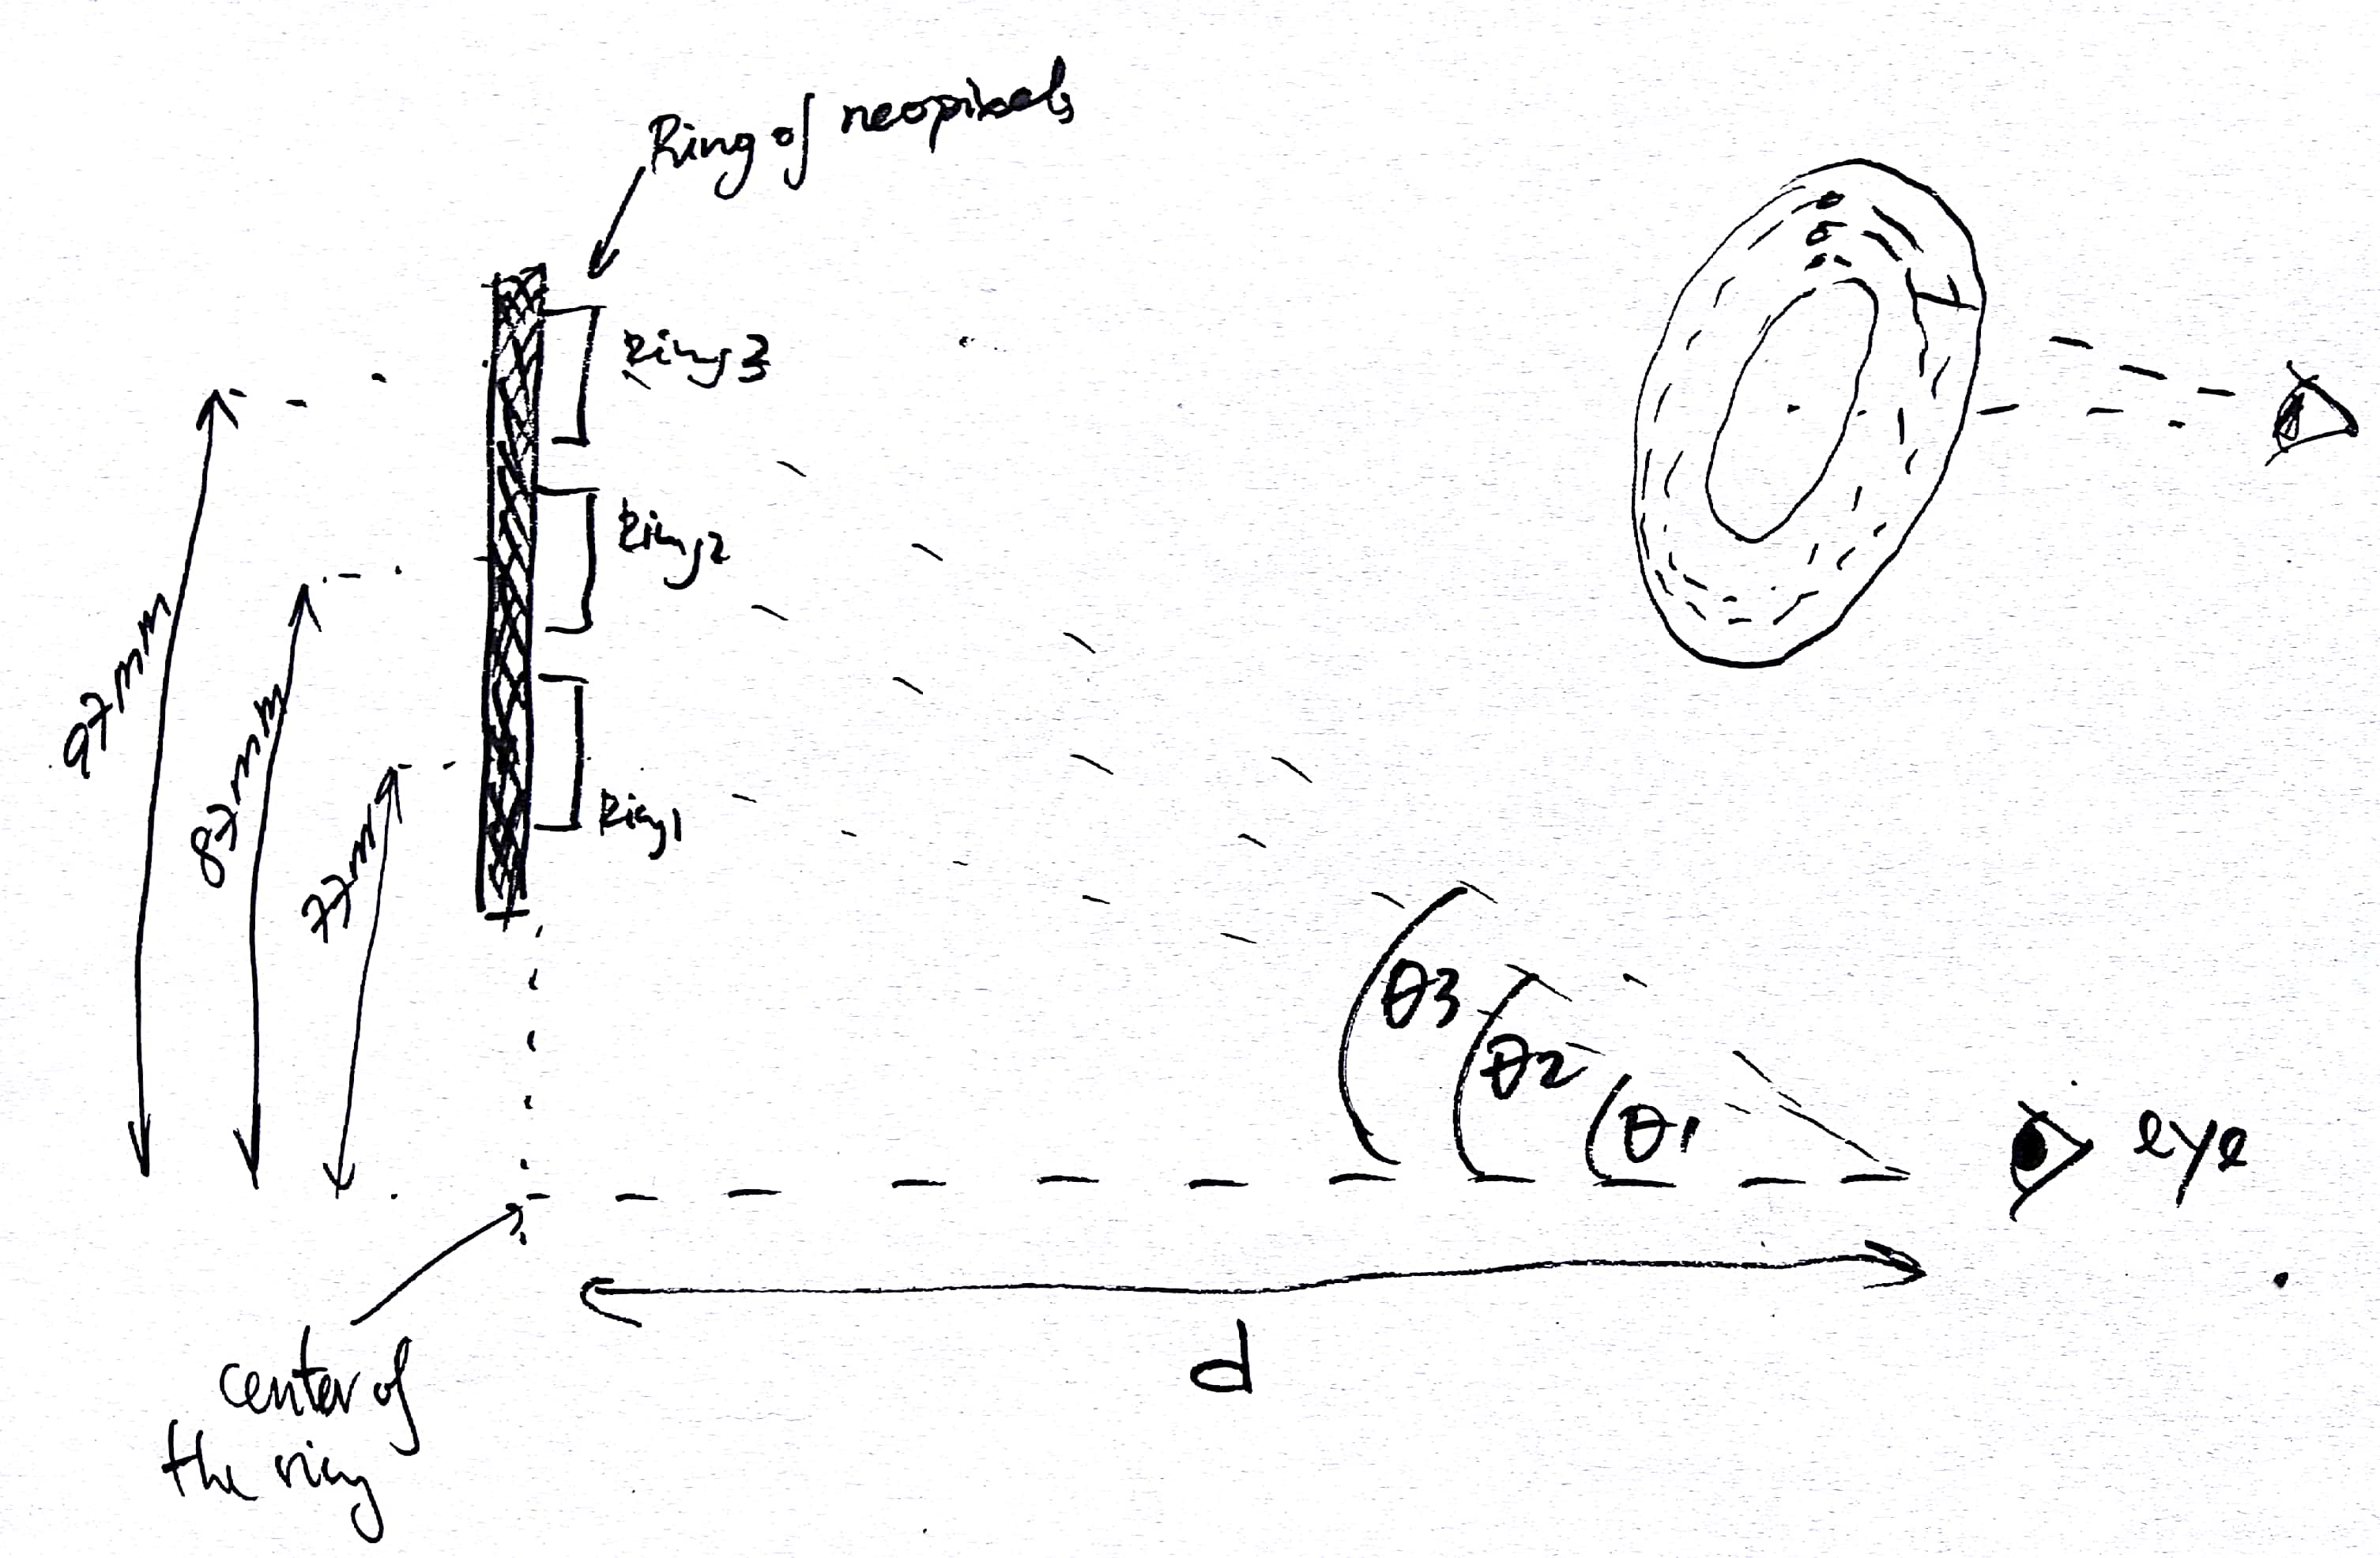
\includegraphics[scale=0.1]{ring_calculation.jpg}
\caption{Relative position of the neopixel rings}
\label{fig:neopixel_ring_dimension}
\end{figure}
Using the dimension from \cref{fig:neopixel_ring_dimension} and the lowest intensity emitted by the blue led, the total illuminace of the rings at a specific distance can be calculated using the following equation:
\begin{equation}\label{eq:total_illuminance}
E_{v_{total}} = N*Ev*(\cos(\theta_1)+\cos(\theta_2)+\cos(\theta_3))
\end{equation}
The result of the calculation are tabulated in the \cref{table:neopixel_illuminance}. The NPSC will not meet the light requirement if the it is placed more than one meter away from the subject.

\begin{table}[h!]
\centering
\caption{Illuminance of the Blue led of neopixel ring for distance ranging from 10cm to 110cm. Result with no angle consieration represent all neopixels in one point while results with angle consideration take into account the relative position of the each pixels to the subject location.}
\label{table:neopixel_illuminance}
\begin{tabular}{ccc}
\hline
\hline
\multirow{2}{*}{Distance (cm)}  & \multicolumn{2}{c}{Illuminance (lux)} \\  
 & no angle consideration & with angle \\
\hline
10 & 3600 & 2715.18\\
20 & 900 & 824.76\\
30 & 400 & 384.02\\
40 & 225 & 219.8\\
50 & 144 & 141.84\\
60 & 100 & 98.85\\
70 & 73.47 & 72.9\\
80 & 56.25 & 55.92\\
90 & 44.44 & 44.24\\
100 & 36 & 35.86\\
110 & 29.75 & 29.66\\
\hline
\hline
\end{tabular}
\end{table}
%%%%%%%%%%%%%%%%%%%%%%%%%%%%%%%%%%%%%%%%%%%%%%%%%%%%%%%%%%%%%%%%%%%%%%%%%%%%%%%%%%%%
% SECTION: Communication protocols
%%%%%%%%%%%%%%%%%%%%%%%%%%%%%%%%%%%%%%%%%%%%%%%%%%%%%%%%%%%%%%%%%%%%%%%%%%%%%%%%%%%%
\section{Communication protocols}\label{com_protocols}
The NPSC requires different integrated circuits using various communication protocols, below is a brief on the use of the protocol required.

\subsection{Serial Peripheral Interface (SPI) Bus}
SPI is a synchronous full duplex serial communication protocol used for short distance communication of electronic devices. With the protocol, one master can communicate to many slaves using a chip select pin (use to select the slave) but a slave can only talk to the master device. SPI uses 4 signals namely, the Master Out Slave In (MOSI), the Master In Slave Out (MISO), the clock (SCK), and the slave select or chip select (SS). Since SPI uses a clock, it does not require the configuration of a baud rate before communication. The main inconvenience with SPI is the number of pins required for a one to one communication, for every additional slave, the master must provide an SS pins which make SPI not the ideal protocol for communicating to multiple slaves devices \cite{spi}. 
\begin{figure}[h!]
\centering
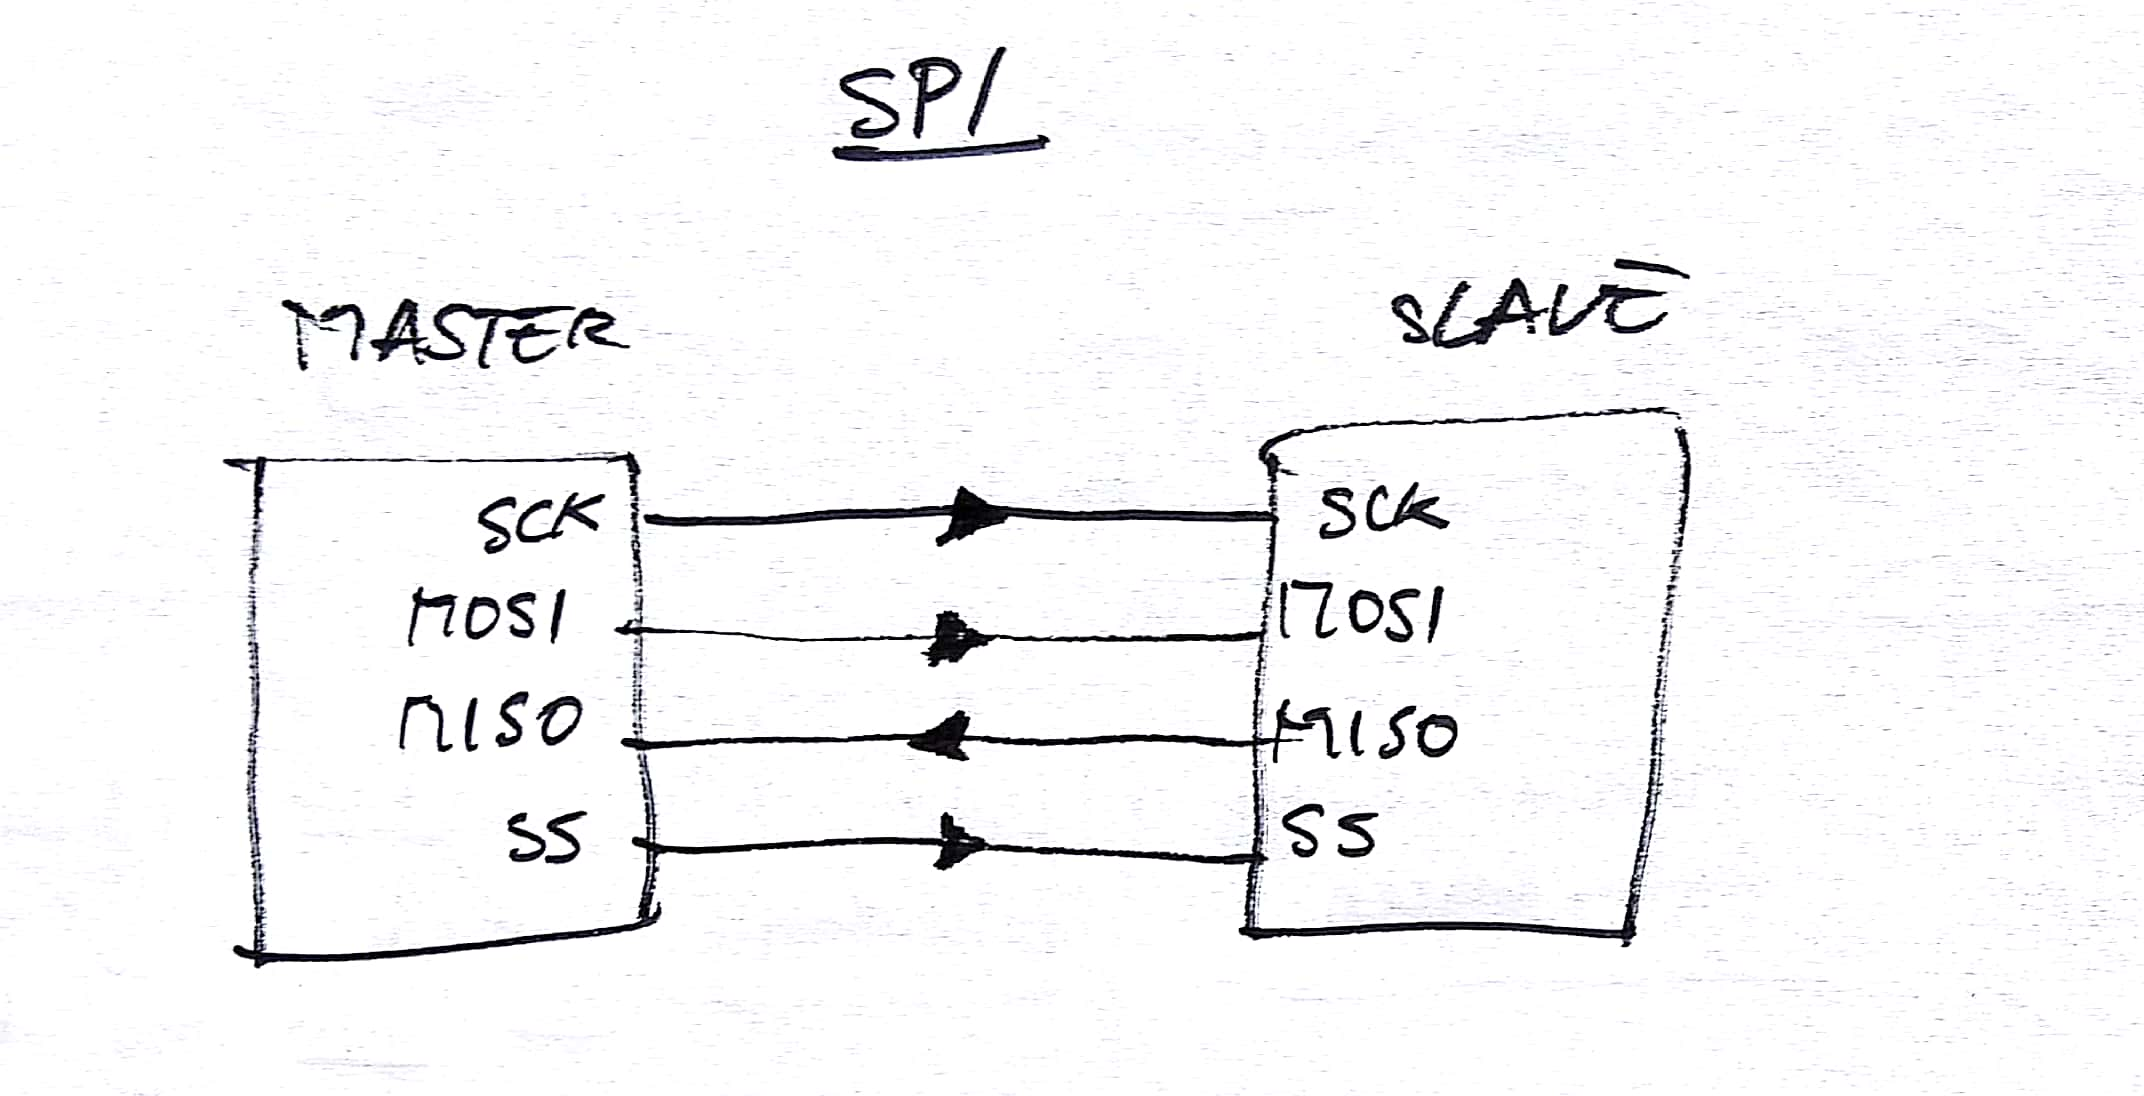
\includegraphics[scale=0.2]{spi.jpg}
\caption{Wire connection setting for SPI communication between a master and a slave device}
\label{fig:spi_coms}
\end{figure}
\subsection{Universal asynchronous receiver-transmitter (UART)}
UART is an asynchronous full duplex communication protocol making use of two signals a transmit signal (TX) and a receive signal (RX). With UART, both devices need to agree on a baud-rate for communication, this rate defines the number of bytes to be sent and received. The problem with UART is the complexity of the protocol required to ensure synchronous communication and correct transfer of information between device. Although theoretically, UART baud-rate is infinite, it is practically limited to 230400 bits per seconds \cite{uart}.   
\begin{figure}[h!]
\centering
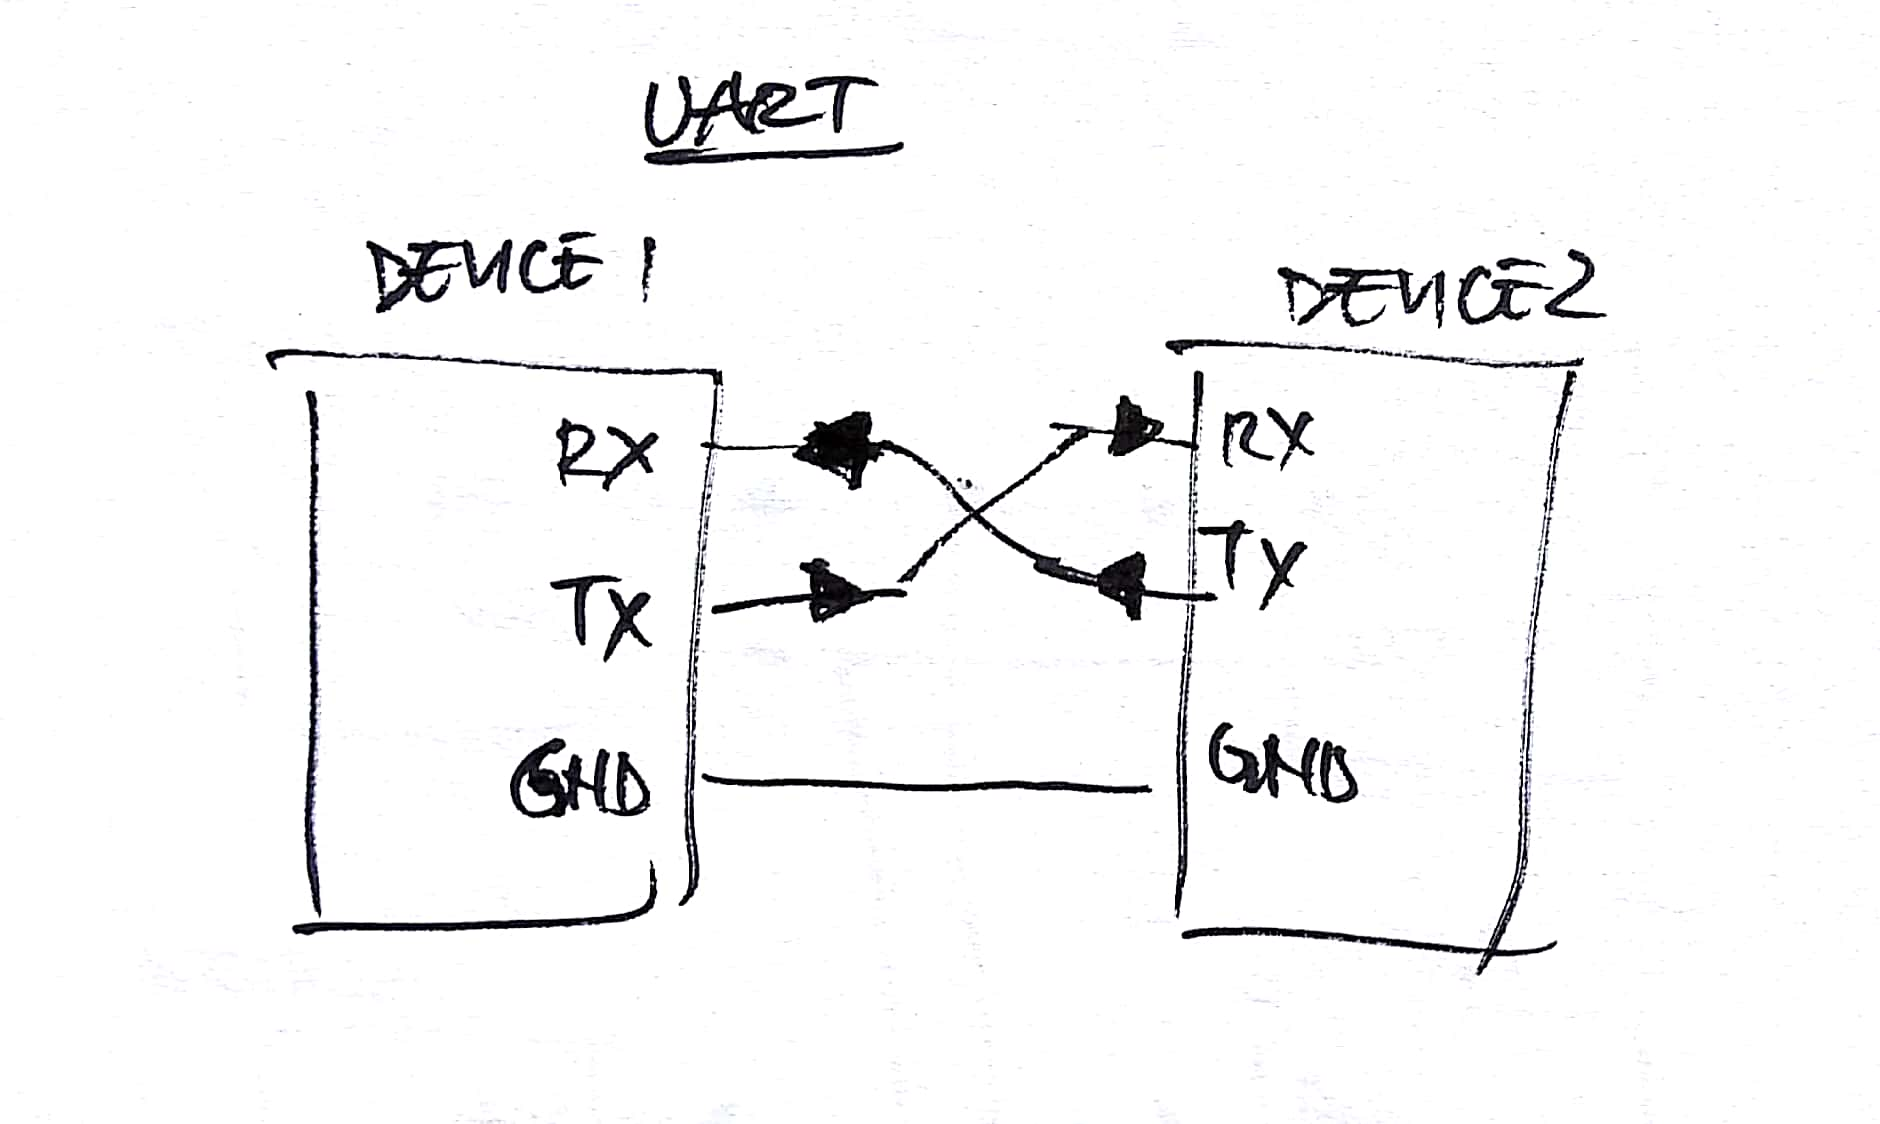
\includegraphics[scale=0.2]{uart.jpg}
\caption{Wire connection setting for UART communication between two devices}
\label{fig:uart_coms}
\end{figure}
\subsection{Inter-Integrated Circuit (I2C)}
I2C is a serial protocol that allows communications from multiple slaves to multiple masters. It takes a bit of both SPI and UART by being designed for short distance communication and requiring only two pins, namely the data line (SDA) and clock line (SCL). Its clock ranges from $100kHz$ to $400kHz$ and a byte is sent at a time. Furthermore, with the I2C protocol, each slave must have a unique address used by the master for communication \cite{i2c}.  
\begin{figure}[h!]
\centering
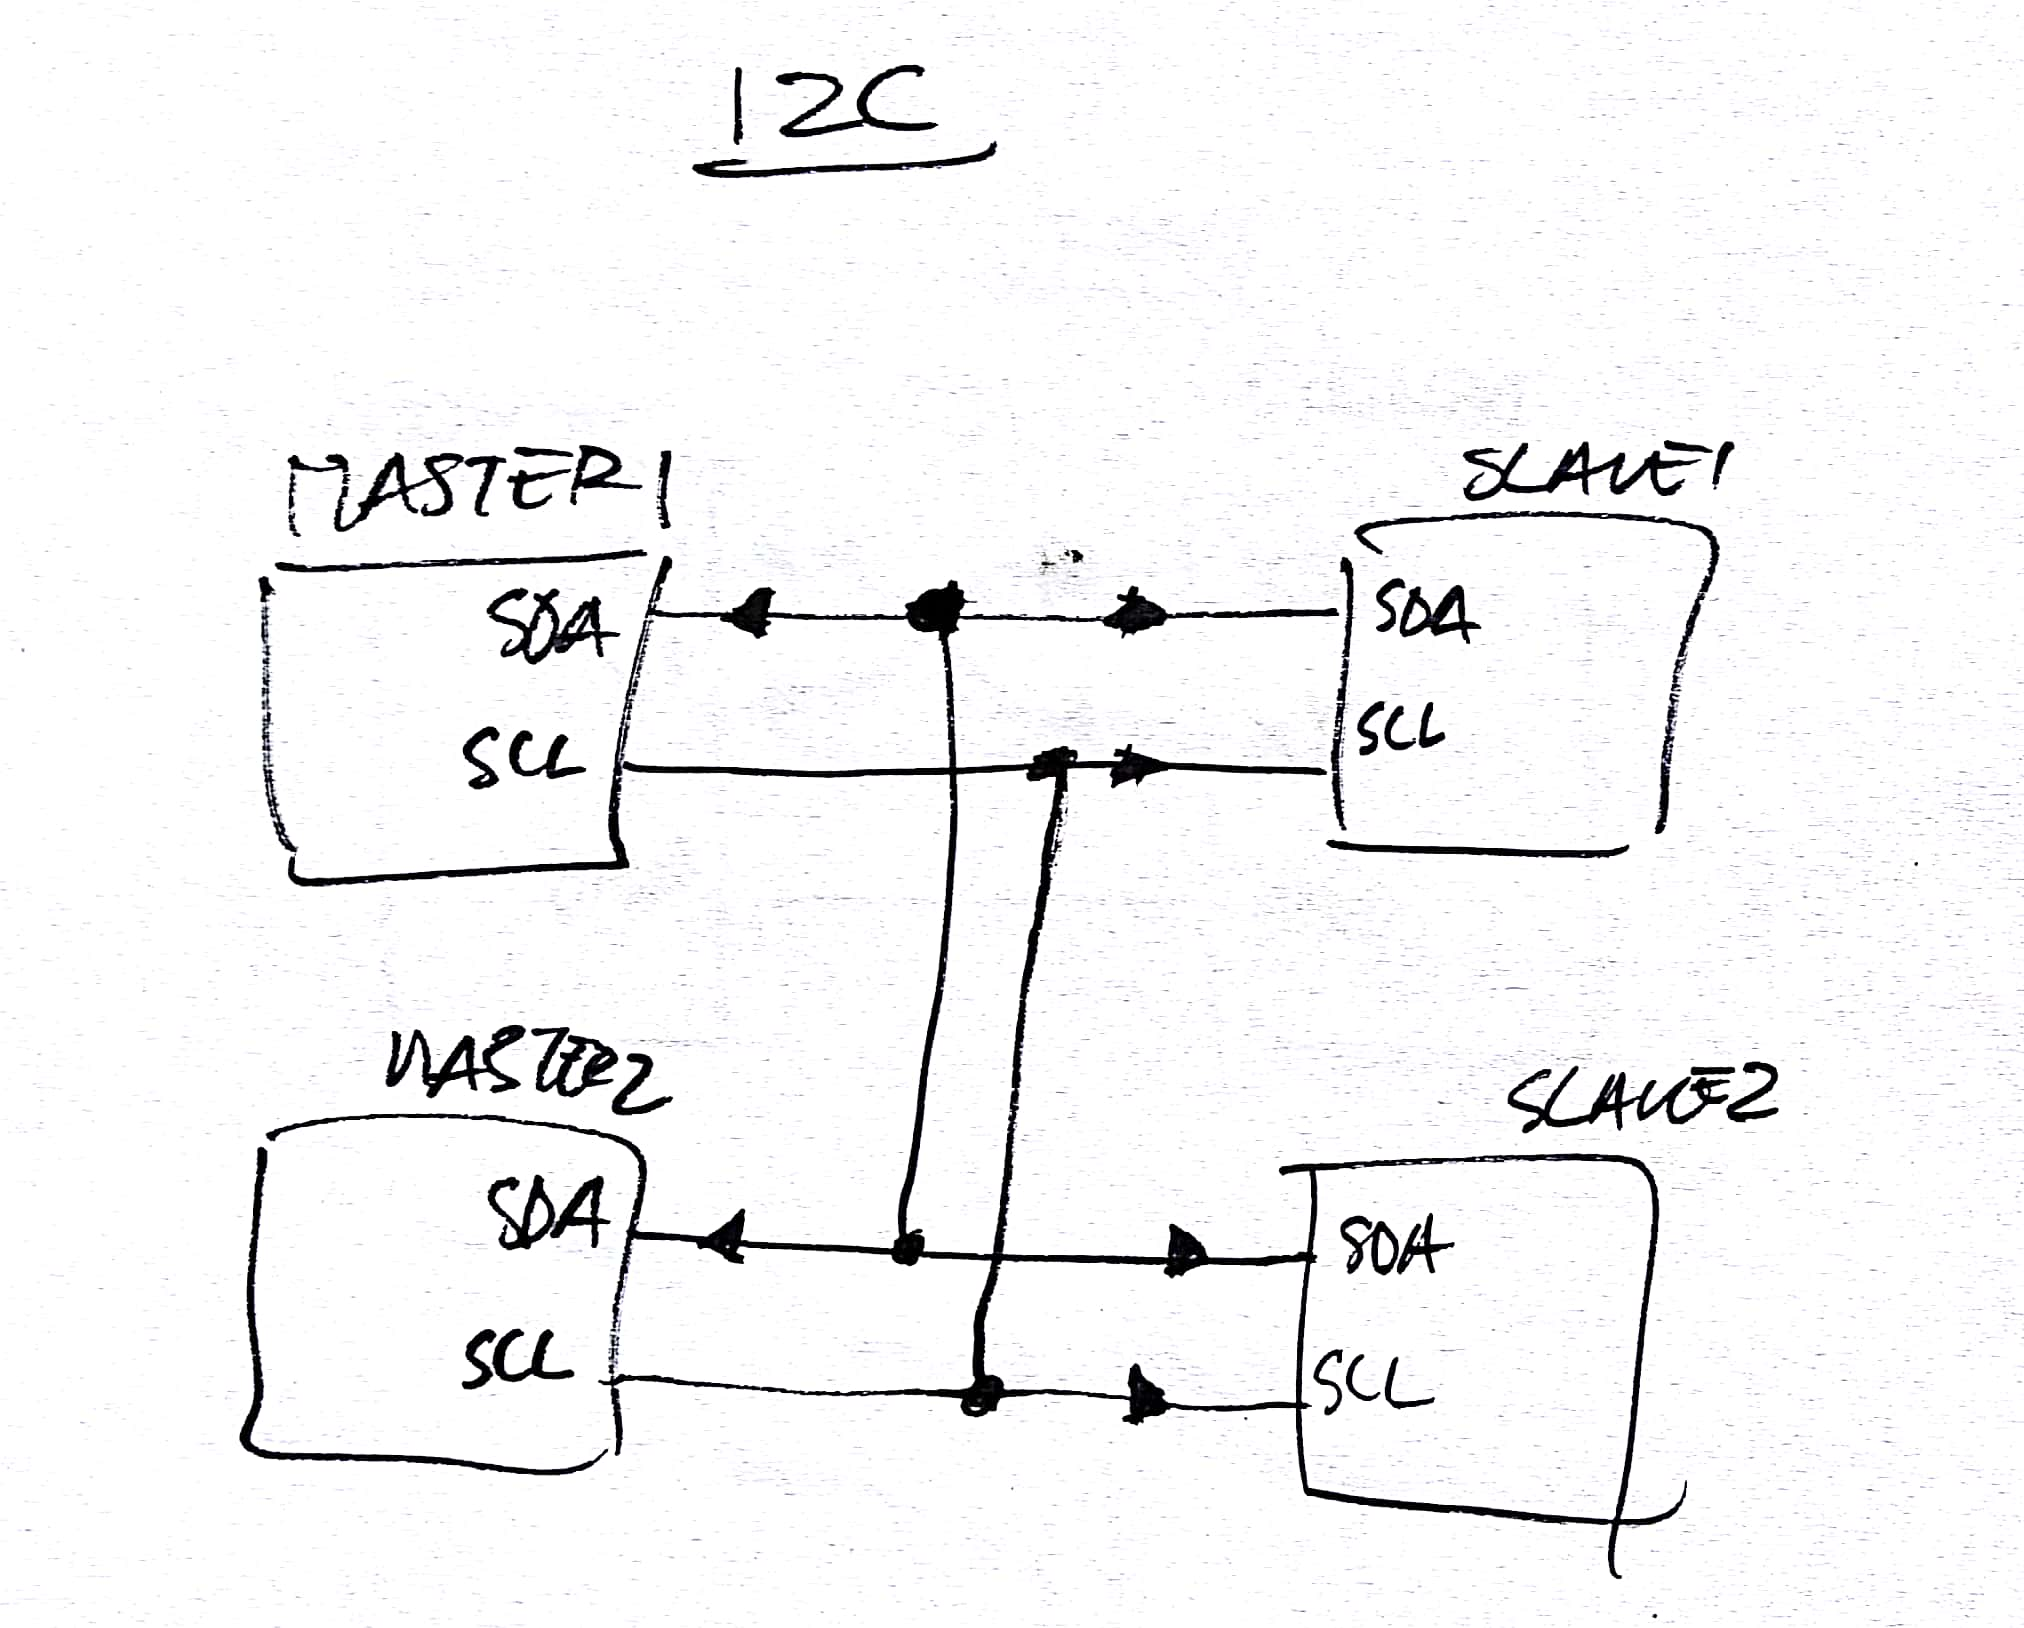
\includegraphics[scale=0.2]{i2c.jpg}
\caption{Wire connection setting for I2C communication between two masters and two slaves devices}
\label{fig:i2c_coms}
\end{figure}
\subsection{Neopixels serial protocol}
Each neopixel has a built-in IC controlling the LEDs' intensity based on the data received. The neopixels use a single wire communication protocol. The neopixels can be connected to form a daisy chain (cascade)\cref{fig:neopixel_cascade} allowing to program of a series of neopixels using one signal. Each neopixel requires 24 Bytes (32 Bytes for RGBW LEDs), each bytes is an encoded bit using a Non-Return-to-Zero encoding \cref{fig:neopixel_nrz}. On receiving a sequence of data, the first neopixel in the chain takes the first 24 bytes and passes the rest of the data to the next neopixel in the daisy chain and so for. This operation continues until a \textit{rest signal} is received by the first neopixel \cref{fig:neopixel_cascade}. This is possible because each neopixel is capable of reshaping the incoming signal preserving the integrity its integrity of continuous transmission.

\begin{figure}[h!]
\centering
\begin{minipage}[b]{0.45\textwidth}
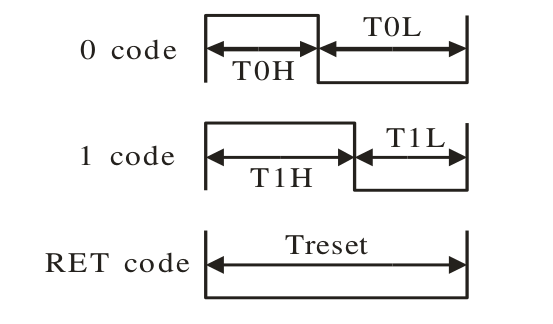
\includegraphics[scale=0.4]{neopixel_nrz.png}
\subcaption[first caption.]{Non-return-to-zero encoding of a single bit in the neopixels programming protocol}
\label{fig:neopixel_nrz}
\end{minipage}
\begin{minipage}[b]{0.45\textwidth}
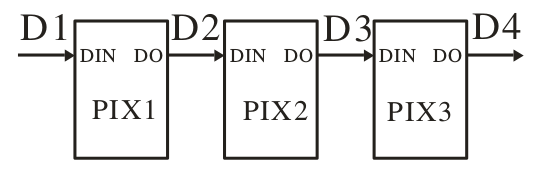
\includegraphics[scale=0.4]{neopixel_cascade.png}
\subcaption[second caption.]{Neopixels connected in daisy chain (cascade).}
\label{fig:neopixel_cascade}
\end{minipage}
\begin{minipage}[b]{\textwidth}
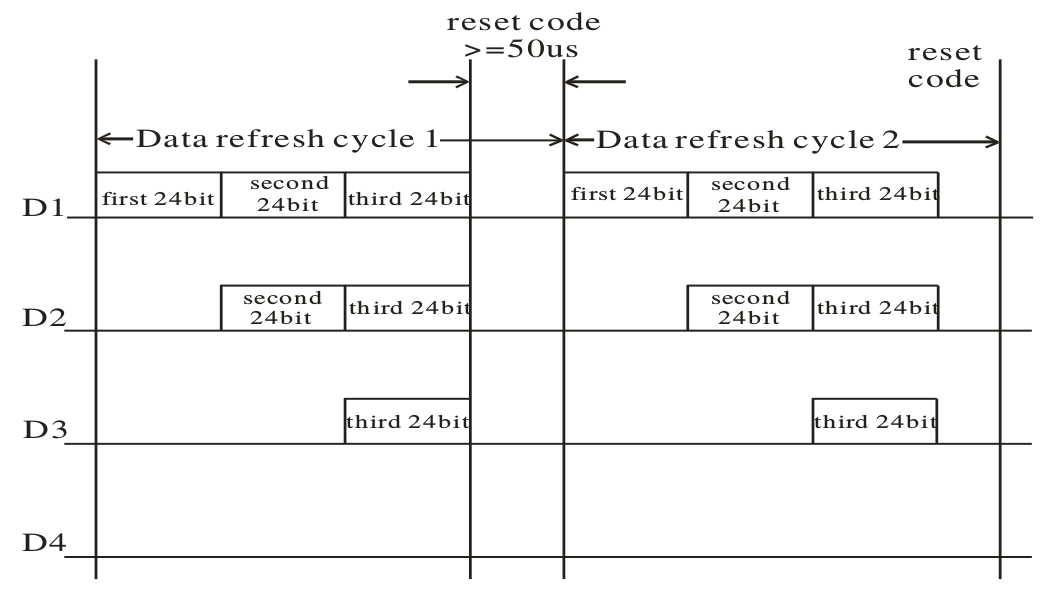
\includegraphics[scale=0.45]{neopixel_serial.png}
\subcaption[third caption.]{As the first neopixel receives a stream of multiple 8 Bytes chunck of data, it takes the first 8 Bytes from the stream and transmit the rest to the next neopixel in the cascade. A rest signal indicates where the stream of data ends.}
\label{fig:neopixel_cascade}
\end{minipage}
\caption{Illustration of the neopixels serial interface}
\label{fig:neopixel_protocol}
\end{figure}
 
%%%%%%%%%%%%%%%%%%%%%%%%%%%%%%%%%%%%%%%%%%%%%%%%%%%%%%%%%%%%%%%%%%%%%%%%%%%%%%%%%%%%
% SECTION: PCB Board Design
%%%%%%%%%%%%%%%%%%%%%%%%%%%%%%%%%%%%%%%%%%%%%%%%%%%%%%%%%%%%%%%%%%%%%%%%%%%%%%%%%%%%
\section{PCB Board Design}\label{PCB_requirement}
Printed Circuit Boards (PCBs) are almost present in every electronic circuit as they hold all the components together and implement the electrical connections. Designing a PCB is a process easily prone to errors, therefore a good PCB design requires the implementation of the design steps. \Cref{fig:pcb_design_flow} illustrates an examples of the ideal pcb design steps. In making the NPSC PCBs these steps give an engineering approach that can be elaborated further based on the PCBs requirement. For example, the designer might question what is the best placement for certain component and thus be referred to some PCBs design standards such as the IPC2221.\\
One important design requirement (need) for the NPSC light requirement is its theoretical current drawn at full pixel brightness. The board-level diagram of the NPSC ring of the neopixel board should therefore be designed so that the track are wide enough to dissipate all the heat evenly across the board. The \textbf{IPC2221}, a generic standard for printed board design published by the \textit{Association Connecting Electronics Industries} \cite{pcb_design} describes a method for finding the mininmal width track given a specific current (see fig 6-4 from the IPC2221 \cite{pcb_design}(pp. 41)). A Javascript program based on the IPC2221 standard can be easily use to determine the track width \cite{pcb_track_width}. This web application use the track cuurent, thickness, temperature rise, ambient temperature and track lenght as input to determine the required track width.      
\begin{figure}[ht]
\centering
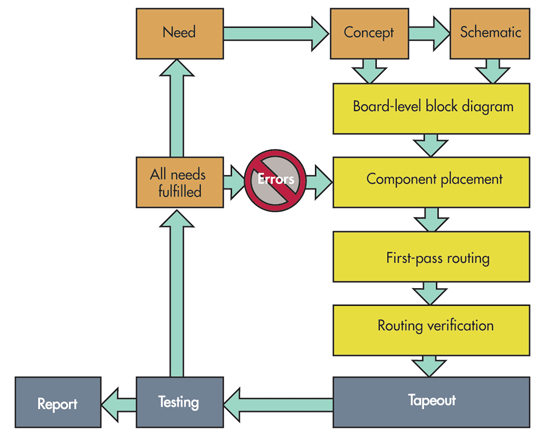
\includegraphics[scale=0.5]{pcb_design_flow.png}
\caption{Ideal PCB design flow, starting from the need, followed by the design, implementation and testing}
\label{fig:pcb_design_flow}
\end{figure}

%%%%%%%%%%%%%%%%%%%%%%%%%%%%%%%%%%%%%%%%%%%%%%%%%%%%%%%%%%%%%%%%%%%%%%%%%%%%%%%%%%%%
% SECTION: Software
%%%%%%%%%%%%%%%%%%%%%%%%%%%%%%%%%%%%%%%%%%%%%%%%%%%%%%%%%%%%%%%%%%%%%%%%%%%%%%%%%%%%
\section{Programming Languages}
Choosing the right programming language for software development is a crutial step, expecially in embedded system design as carefull manipulation of memory is required. The languages below are the ones chosen for the development of NPSC. 
\subsection{C}
\textit{C} is a mid-level programming language \footnote{has the advantages of both ligh and low level language} providing the ability to get close to the hardware while keeping some abstract layers for programming \cite{c_programming}.It has an easy and straight forward syntax compared to languages such as Java, C has accumulated a lot of support and has lots of functions and documentation. Although C does not support Object Orientated Programming, it is a Procedure Orientated Language (POL) which means it is designed to create programs that follow an algorithm. This latter feature of C make it the favourite programming language for Embedded System. 

\subsection{C++}
\textit{C++} is a programming language based on C which has higher level functionality. In the context of this project, C++ is used to test the functionality of the NPSC modules using an Arduino.

%%%%%%%%%%%%%%%%%%%%%%%%%%%%%%%%%%%%%%%%%%%%%%%%%%%%%%%%%%%%%%%%%%%%%%%%%%%%%%%%%%%%
% SECTION: Software Tools and Libraries
%%%%%%%%%%%%%%%%%%%%%%%%%%%%%%%%%%%%%%%%%%%%%%%%%%%%%%%%%%%%%%%%%%%%%%%%%%%%%%%%%%%%
\section{Software Tools and Libraries}
Developing an embedded system software can be quite frustrating, for this reason tools with decent debugging features and programming interface should be chosen to reduce development to its minimal. 

\subsection{Atollic TrueSTUDIO for ARM}
Atollic TrueSTUDIO is an IDE based on Eclipse. It comes with the GCC toolchain for ARM and with debugging features beuilt on top of GDB. It has more advanced features compared to Eclipse in the development embedded system application. Its debugging features include the use of any debug probe compatible with the GDB-server, P\&E Micro, SEGGER J-Link / J-Trace, ST-Link, OpenOCD are all supported by Atollic TrueSTUDIO. It supports debugging of single and multi core devices and allows real time view of memory mapping, peripheral registers, advanced visualisation of variable and complex break point, CPU fault analysis and many more. Another important debugging feature of Atollic TrueSTUDIO is the instruction tracing and system analysis real time event analysis of Real Time Operating System \cite{atollic}.

\subsection{Nextion IDE}\label{nextion}
Nextion IDE is the official IDE designed for programming any Nextion HMI touch-screen. The IDE allows the designed and programmation of a GUI interface and the definition of serial commands to be sent to a MCU. Nextion IDE is designed to reduce significantly development time of touch-screen interface in an embedded system project \cite{nextion}. 

\subsection{MIT App Inventor 2}


%%%%%%%%%%%%%%%%%%%%%%%%%%%%%%%%%%%%%%%%%%%%%%%%%%%%%%%%%%%%%%%%%%%%%%%%%%%%%%%%%%%%
% SECTION: Design Models
%%%%%%%%%%%%%%%%%%%%%%%%%%%%%%%%%%%%%%%%%%%%%%%%%%%%%%%%%%%%%%%%%%%%%%%%%%%%%%%%%%%%
\section{Design Models}
Designing an embedded system requires the use of suitable design methods. This section describes the different design models used for the project.

\subsection{V-Model}
The V-Model is a linear product-development methodology composed of two main parts. On the left side of the diagram (see \cref{fig:v_model} ) is the project definition. On that branch, the requirements are defined, the system design, architectural design and module design are performed. At the bottom of the diagram is the implementation of the design. Following the implementation is the project testing and integration. The project testing starts with the unit testing of the module design followed by integration testing in which the architectural design is tested to ensure that the system functions well across all components. The next step consists of the system testing and the validation of the performance defined in the design. The last step is the acceptance testing, done to ensure that the system can be deployed.       
\begin{figure}[ht]
\centering
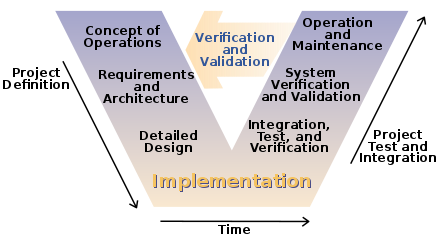
\includegraphics[scale=0.7]{v_model.png}
\caption{V-Model basic template used for system definition and testing}
\label{fig:v_model}
\end{figure}

\subsection{Spiral Model}
The Spiral model is a combination of the iterative model \footnote{Cyclic process consisting of design, prototyping, testing, analysis and refinement of a product} and the waterfall model \footnote{linear sequential process consisting of conception, initiation, analysis, design, construction, testing, deployment and maintenance of a product.} through which a product can be refined after each cycle. \Cref{fig:spiral_model} illustrate the order of the spiral model steps. The first step is the identification, it consists of identifying the user, system, sub-system, and unit requirements. The second step consists of the system, architectural, physical design and logical design of all modules. The prototype is built during the third step, the prototype serves as a proof of concept. During the last stage, the prototype performance is evaluated as well as the validation of the system requirements. Moreover, a risk and cost analysis alongside with the overall feasibility of the project is evaluated at this stage.  
\begin{figure}[ht]
\centering
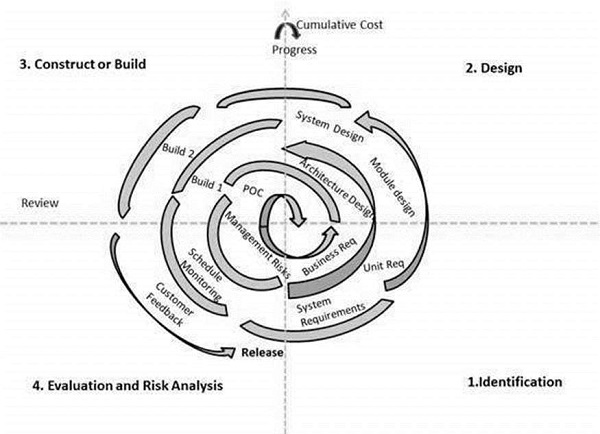
\includegraphics[scale=0.7]{spiral_model.jpg}
\caption{Spiral-Model basic template used for system refinement}
\label{fig:spiral_model}
\end{figure}